\documentclass{sig-alternate}
\usepackage{algorithm}
\usepackage{algorithmic}
\usepackage{graphicx}
\usepackage{epsfig}
\usepackage{color}
\usepackage{amssymb}
\usepackage{amsmath}
\usepackage{flushend}
\usepackage{cite,float}
\usepackage[normalem]{ulem}
\usepackage{verbatim}
%\usepackage{subfig}
\usepackage{subfigure}

%\newtheorem{theorem}{Theorem}[section]
\newtheorem{theorem}{Theorem}
\newtheorem{lemma}{Lemma}[section]
\newtheorem{axiom}{Axiom}
\newtheorem{proposition}[theorem]{Proposition}
\newtheorem{definition}{Definition}[section]
%
%\newcounter{defCount}
%\newenvironment{definition}[1][Definition]{
%    \refstepcounter{defCount}
%    \begin{trivlist}
%    \item[\hskip \labelsep
%        {\bfseries Definition \arabic{defCount} #1}]}
%    {\end{trivlist}}

\newcounter{coroCount}
\newenvironment{corollary}[1][]{
    \refstepcounter{coroCount}
    \begin{trivlist}
    \item[\hskip \labelsep
        {\bfseries Corollary \arabic{coroCount} #1}]}
    {\end{trivlist}}

\newenvironment{example}[1][Example]{\begin{trivlist}
\item[\hskip \labelsep {\bfseries #1}]}{\end{trivlist}}
\newenvironment{remark}[1][Remark]{\begin{trivlist}
\item[\hskip \labelsep {\bfseries #1}]}{\end{trivlist}}

\newcommand{\eat}[1]{}

\begin{document}

\title{Efficient Evaluation of Skyline Queries in Wireless Data Broadcast Environments}

\numberofauthors{2}

\author
{
 \alignauthor Chih-Jye Wang\\
 \affaddr{Dept. of Computer Science and Software Engineering}\\
 \affaddr{Auburn University}\\
 \affaddr{Auburn, AL 36849, USA}\\
 \email{wangchj@auburn.edu}
 \alignauthor Wei-Shinn Ku\\
 \affaddr{Dept. of Computer Science and Software Engineering}\\
 \affaddr{Auburn University}\\
 \affaddr{Auburn, AL 36849, USA}\\
 \email{weishinn@auburn.edu}
}

\conferenceinfo{GIS'12,} {November 6-9, 2012. Redondo Beach, CA,
USA}\CopyrightYear{2012}

\maketitle

\begin{abstract}
Skyline is a popular query type which retrieves data objects that
are not dominated by any other object with respect to multiple
attributes. Skyline queries have broad applications; however,
limited studies have been done on skyline in the broadcast data
model. No study has been done on flexible skyline query
evaluations in this model that can handle a combination of minimum
and maximum attributes. In this paper, we propose the depth-first
distributed index (DFDI) and the skyline algorithms that
incorporate DFDI to efficiently evaluate skyline in broadcast
environments. Our extensive simulations show that the proposed
algorithms can answer skyline queries in broadcast environments
effectively and efficiently.
\end{abstract}

\category{H.2.8}{Database Management}{Database
Application}[Spatial databases and GIS]

\terms{Algorithms and Experimentation}

\keywords{Data broadcast, Skyline query, Location-based services.} % NOT required for Proceedings

\section{Introduction}\label{sec-intro}

Skyline is a query operation that retrieves data items which are
considered ``interesting objects'' with respect to multiple
attributes of the data set. For example, someone who is planning
for an ocean-view vacation would be interested to find a list of
hotels that are close to the ocean and at the same time not too
expensive. A hypothetical data set of hotels is shown in
Table~\ref{tab:sample_data}. The two relevant attributes in this
case are \emph{minimum distance} to the ocean and \emph{minimum
price}. Figure~\ref{fig:skyline} shows the skyline points in solid
dots as the operation finds hotel records that are successively
further from the ocean, but the prices are the best for such
distances. In the figure, hotel $a$ is a skyline point because it
is closest to the ocean, although it is not the lowest price.
Hotels $b$ and $d$ are part of the skyline because each have the
closest distance at its price. Hotel $k$ is a skyline point
because it is the cheapest of all hotels.

\begin{figure}[h]
\centering \subfigure[2-D skyline of hotels of (X = min, Y = min)]{
    \includegraphics[width=1.5in]{Figures/skyline_points.eps}
    \label{fig:skyline}
} \subfigure[3-D skyline of stocks with attributes (X = min, Y = min, Z = max)]{
    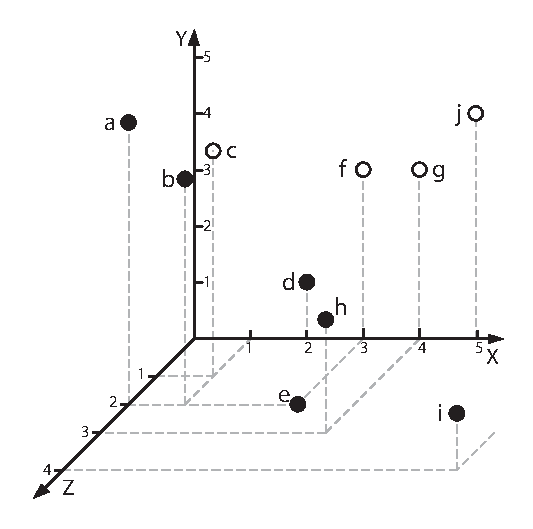
\includegraphics[width=1.5in]{Figures/skyline_points_3d.eps}
    \label{fig:skyline_points_3d}
} \caption{Sample Skylines}
\end{figure}

\begin{table}[b!]
  %\vspace*{-10pt}
  \centering
  \caption{Sample Data}
  %\vspace*{5pt}
  \label{tab:sample_data}
  \subfigure[\small 2-d Data of Fig 1(a)]{
  \label{tab:sample_data_a}
  \begin{tabular}{|c|c|c|}
  \hline
  {\bf Hotel} & {\bf Distance} & {\bf Price} \\ \hline\hline
  a & 1 & 8\\
  b & 2 & 6\\
  c & 4 & 7\\
  d & 3.5 & 3\\
  e & 5 & 4\\
  f & 6 & 7.5\\
  g & 7 & 6\\
  h & 7.5 & 8\\
  i & 6.5 & 3\\
  j & 8 & 4\\
  \hline
  \end{tabular}
  }
  \subfigure[\small 3-d data of Fig 1(b)]{
  \label{tab:sample_data_b}
  \begin{tabular}{|c|c|c|c|}
  \hline
  {\bf Symbol} & {\bf Price} & {\bf P/E} & {\bf Yield} \\ \hline\hline
  a & 0 & 5 & 2\\
  b & 1 & 4 & 2\\
  c & 1 & 4 & 1\\
  d & 2 & 2 & 0\\
  e & 3 & 0 & 2\\
  f & 3 & 3 & 0\\
  g & 4 & 3 & 0\\
  h & 4 & 2 & 3\\
  i & 7 & 1 & 4\\
  j & 5 & 4 & 0\\
  \hline
  \end{tabular}
  }
\end{table}


Skyline has broad applications and relevance due to multi-criteria
benefit. Skyline computation in realtime streaming systems with
frequent data updates has been studied in~\cite{Lin05stabbingthe}
and~\cite{Tao06maintainingsliding}. For distributed web services,
skyline query solutions have been proposed
in~\cite{Balke04efficientdistributed}. Skyline query has also been
applied in sensor networks
in~\cite{Seong:2009:ESQ:1644993.1645022}. Meanwhile, the data
broadcast is a scalable way to disseminate data (e.g., FM
broadcasting). Unlike the on-demand model, such as most of the
services on the Internet, the broadcast model can scale almost
indefinitely. A challenge and drawback of this model is the
forward-only access characteristic. While many studies have been
done on different query types to support efficient query
evaluation in broadcast
environments~\cite{DBLP:journals/tmc/KuZW08,dsi,DBLP:conf/cikm/Hara02},
to the best of our knowledge, the work
in~\cite{Ha:2009:EEP:1616994.1617050} is the only study on skyline
query processing in broadcast environments.
Although~\cite{Ha:2009:EEP:1616994.1617050} considers broadcast
efficiency (more details in Section~\ref{sec:wireless_broadcast}),
the proposed solution is unable to support all possible skyline
types (i.e., combinations of min and max attributes) and the work
did not address skyline of higher data dimension ($>2$ dimensions)
as illustrated in figure~\ref{fig:skyline_points_3d}. To address
these challenges, we design a flexible broadcast index and a
skyline evaluation algorithm that utilizes the index to
efficiently evaluate skyline queries. Specifically, our
contributions of this research are as follows:

%In broadcast environment, the clients listens on the broadcast for data records and evaluates
%the skyline queries from the records. The challenge is the forward only data model. A goal
%of this research is to incorporate necessary structure in the broadcast data to help client
%prune unnecessary data.

%While many studies have been done on efficiently evaluating skyline operation in traditional
%database systems, in the best of our knowledge, only one study has been done on skyline
%evaluation in broadcast system. \cite{Ha:2009:EEP:1616994.1617050} proposed encoding
%the data records using Sweep space-filling curve (SFC) over relevant attributes before
%broadcasting the system.
%as shown in Figure \ref{fig:SFC}.
%Since the encoding process decides
%a specific skyline application,
%such that the encoding can be used for the MINIMUM skyline operation on all attributes, such
%encoding and broadcast is not flexible to support different kinds of application from the
%broadcast program. In addition SFC encoding is inflexible in data with more than two dimensions.

%In this paper, we propose a flexible technique for evaluation of skyline in broadcast environment.
%Our technique is a general indexing technique that can easily incorporate different index structures,
%such as the R-Tree and the KD-Tree\cite{Bentley:1975:MBS:361002.361007}, into the index structure
%to facilitate evaluation on broadcast
%program. An advantage of this flexibility is that for data of high dimension, the system can use
%KD-Tree, while data of low dimension (two or three), R-Tree can be an efficient choice. Our solution
%is based on pruning region concept and does not restrict the skyline operation to either MAX or
%MIN. The client is able to choose between these two criteria on any of the attributes of the data.

\begin{itemize}
\item We design a flexible on air index that supports skyline
query evaluation in data broadcast environments for arbitrary
number of data dimension.

\item We propose an efficient data broadcast skyline query
algorithm that handles both min and max attributes.

\item We evaluate the performance of the proposed algorithms
through extensive experiments.
\end{itemize}

The rest of this paper is organized as follows. Section 2 provides
background knowledge of the skyline operator and wireless data
broadcast. We introduce our index structures to facilitate
broadcast skyline query in Section 3. In Section 4 we propose our
pruning region based technique for skyline query evaluation. The
experimental validation of our design is presented in Section 5.
Section 6 surveys related works. We conclude the paper with a
discussion of future work in Section 7.


\section{Preliminary}\label{sec-prelim}

\subsection{Skyline Query}\label{sec:skyline_operator}

Skyline query is an operation that finds all data records which
are not dominated by any other data objects in a given data set.
Skyline query is closely related to the maximal vector
problem~\cite{Kung75onfinding,conf/vldb/GodfreySG05}. Here, we
briefly introduce these concepts.

%define the terms that are used to formally define maximal vectors
%and skyline operator. The concept of \emph{attribute domains},
%though intuitive, is also defined here and will be used to
%formally define \emph{pruning region}, which is the core idea used
%in the solution section of this paper.

%We use $n$ to denote the number of dimension of the skyline query,
%and only consider attributes in the data set that are interested
%for skyline query. Non-skyline attributes are only used for
%clarification of illustrations.

%\begin{definition}[Record] Given the set of domains of totally
%ordering sets $D$ = \{$D_1$, $D_2$, ... $D_n$\} and a set of
%attributes $A$ = \{$A_1$, $A_2$, ... $A_n$\}, a records, denoted
%by $p$, is a n-tuple $p$ = ($A_1$, $A_2$, ... $A_n$) such that
%$A_i$ $\epsilon$ $D_i$ for $i$ = 1 to $n$.
%\end{definition}

%\begin{definition}[Data Set]
%Data set, denoted by $P$ is a set of data records denoted by $P$ =
%\{$p_1$, $p_2$, ..., $p_m$\}, where $m$ is the number of tuples in
%the data set.
%\end{definition}

%Figure~\ref{tab:sample_data} shows an example of a data set where
%the domain of the first attribute is alphabets; the domain for the
%second and the third attribute is the set of positive real
%numbers, $\mathbb{R}^+$.

%The skyline operation has been known as the problem of
%finding maximal vectors from a set of vectors as
%studied in \cite{Kung75onfinding}. Maximal vectors are defined as  follows:

\begin{definition}[Maximal Vector]\label{def:max_vector}
Given the set of vectors $P$, for all vectors $v$ $\epsilon$ $P$,
there does not exist $u$ $\epsilon$ $P$ such that $u$ $\geq$ $v$,
then $v$ is a maximal vector.

\begin{equation}\label{eq:max_vector}
    MaxVect(P) = \{v | \forall v, u \epsilon P \nexists u \geq v\}
\end{equation}

\end{definition}

The comparison operator $\geq$ used in
Equation~\ref{eq:max_vector} is defined on vectors such that for
two vectors $u$, $v$ $\epsilon$ $V$, $u$ $\geq$ $v$ if $u_i$
$\geq$ $v_i$ for $i$ = 1 to $n$. Vice versa for the $\leq$
operator. In other words, a vector $v$ is ``greater than" the
other vector $u$ if and only if all elements of $v$ is ``greater
than or equal to'' all elements of $u$. The comparison operators
for each element of the vectors are the natural ordering operators
defined on each domain.

The only difference between the maximal vector operation defined
in definition \ref{def:max_vector} and the skyline operation is
that the skyline operator defines a set of \emph{preference
specifiers}, $\sigma$, which are to be either \emph{MIN} or
\emph{MAX} for each attribute.

%In addition, the skyline operator defines the preference specifier for
%each relevant skyline attribute. The preference specifiers, $\sigma$,
%is a set of Minimize (MIN) or Maximize (MAX) specifiers that defines
%the dominance relationship on each attribute. For a attribute with a
%MIN specifier, a lower value from the domain of the attribute dominates
%a higher value.

%The $\geq$ operator is defined based on the ordering
%of the domain. We redefined the $\geq$ operator to be the
%dominance relationship. In this case, skyline can be defined
%using the finding maximal vector problem.

\begin{definition}[Skyline Operator]\label{def:skyline}
Give a set of tuples, $P$, and an ordered set of preference
specifiers, $\sigma$, the skyline operator is defined as follows:

\begin{equation}\label{eq:skyline}
    Skyline(P, \sigma) = MaxVect(P)
\end{equation}

\end{definition}

In definition~\ref{def:skyline}, the dominance relationship is
defined as follows:

\begin{definition}[Dominance Relationship]\label{def:dom_rel}
Give two points $p_1$ and $p_2$ in $P$, $p_1$ dominates $p_2$, if
and only if all elements of $p_1$ dominates or is equal to all
elements of $p_2$ and at least one element is dominant. Dominance
for each element depends on the preference specifier, $\sigma_i$,
for that attribute. Given $x$ and $y$ from $D_i$, the domanance
for the elements is defined as follows:

\begin{enumerate}
\item If $\sigma_i$ = \emph{MIN}, $x$ {\bf dominates} $y$ if $x$
$<$ $y$. \item If $\sigma_i$ = \emph{MAX}, $x$ {\bf dominates} $y$
if $x$ $>$ $y$.
\end{enumerate}

\end{definition}

\begin{corollary}\label{co:dom_rel}
The dominance relationship is transitive, non-reflexive, and
non-symmetric.
\end{corollary}

\begin{proof}
All three properties can be proven based on the fact that the values of
each attribute domain are ordered: an attribute $x$ is better than $y$ then,
$y$ is worse than $x$. The transitive property of the dominance relationship
follows
from Definition~\ref{def:dom_rel}, if record $A$ dominates $B$ then all
attributes of $A$ are equal or better and there is at least one attribute
that is better; therefore, $B$ dominates $C$ implies that all attributes
of $A$ is
equal or better than $C$ therefore, the relationship is transitive.
The relationship is non-reflexive since if all attribute of $A$ is equal
or better than attribute of $B$ then the ordering of the values of each
attribute domain imply that $B$ does not dominate
$A$. Similarly, $D$ does not dominate itself since the definition states
that at least one must be better for a record to dominate another.
\end{proof}

Following the non-reflexive property of Corollary~\ref{co:dom_rel}, given
two record $A$ and $B$ and $A = B$, if $A$ is a skyline record, then
$B$ is also a skyline record.

Extension SQL syntax for skyline was defined by B\"{o}rzs\"{o}nyi,
et al. in \cite{skyline_operator} as illustrated in Figure
\ref{fig:skyline_sql}. The syntax defines an additional SKYLINE
clause in SQL that specifies how the skyline operation should be
performed. In the SKYLINE clause, relevant attributes (such as
H.price and H.dist in the figure) can be listed. For each
attribute, the syntax defines three attribute specifiers, MIN,
MAX, and DIFF, that tells the operator how each attribute is to be
handled. MIN and MAX denote that the values of the attribute
should be minimized or maximized. DIFF denotes that the values
should be different. The MIN and MAX specifiers are considered in
this paper and in designing our solution. DIFF is not discussed in
this paper.

\begin{figure}[h]
\begin{center}
\line(1,0){240}
\begin{verbatim}
SELECT H.name, H.price, H.distance
FROM H
SKYLINE OF H.price MIN,
H.dist MIN ORDER BY H.name
\end{verbatim}
\line(1,0){240} \caption{\small Skyline SQL Clause.
\label{fig:skyline_sql}}
\end{center}
\end{figure}

%Connecting skyline operator to the maximal vector problem, the set of vectors $V$ represents a
%data set. Each vector, $v$ represents a tuple and each element $v_i$ represents an attribute
%value in a tuple. In the definition of relational database, a data set is represented by a table.
%Each tuple is a row in the table, and each element is an attribute.

%\begin{mydef}[Skyline Operator] Give a set of tuples, $P$, the
%    skyline operator is defined on skyline attributes:
%    \begin{equation}\label{eq:skyline}
%        Skyline(P) = MaxVect(P)
%    \end{equation}
%\end{mydef}

Skyline constraint regions is introduced in
\cite{Ha:2009:EEP:1616994.1617050}. Constraint region limits the
skyline queries to a subset of the data set, instead of the entire
data set. For example a constraint could be a limit of hotel price
within \$100 - \$150 and the distance within 0 to 1 mile from the
beach. Constraint region is a separate issue in skyline queries
that can be easily satisfied with a filtering step to remove all
tuples not in the region preceding the main skyline algorithm. In
this paper, we do not consider constraint region, and assume the
entire space of the data set as the search space.
%The constraint defines a region in
%the graphical representation of the data. If there is no constraint
%region defined, the constraint region is defined to be the entire
%search space. This paper assume that the entire data set as the
%constraint region.

\begin{table}[h]
\centering
\caption{Summary of Analytical Notations} \label{tab:index_attr}
\begin{tabular}{c|l}
\hline
{\bf Notation} & {\bf Description}\\
\hline
$n$ & Number of dimensions of skyline\\
$m$ & Number of records in data set\\
$D$ & A set of attribute domains $D$ = \{$D_1$, ..., $D_n$\}\\
$P$ & A set of records (a set of tuples)\\
$p$ & A record (a n-tuple)\\
$S$ & A set of skyline points\\
$\sigma$ & A set of skyline preference specifier\\
$R$ & A pruning region\\
$B$ & A minimal bounding box (MBR)\\
$E$ & An R-Tree index entry (MBR, time)\\
$b$ & Branching factor of an index tree\\
$h$ & Height of an index tree\\
$L$ & Tree level (1 to $h - 1$). $L = h + 1$\\
$L_r$ & Levels of index tree replication\\
$\rho$ & Index Percentage\\
$\alpha$ & Initial Index Prob\\
$\beta$ & Tuning Time\\
$\gamma$ & Access Time\\
$\iota$ & Space of index (bytes)\\
$\theta$ & Size of the data set (bytes)\\
$\alpha$ & Space of the entire program cycle (bytes) $\iota + \theta$\\
\hline
\end{tabular}
\end{table}

\begin{comment}
\begin{mydef}[Constraint Skyline] Give a set of spatial constraints
    $C$ = \{$c_1$, $c_2$, ..., $c_n$\}
    \begin{equation}
    ConsSkyline(P) = Skyline(P), \\where p \epsilon P~satisfies~C
    \end{equation}
\end{mydef}
\end{comment}


\subsection{Wireless Broadcast}\label{sec:wireless_broadcast}
A wireless broadcast environment consists of a broadcast channel,
a broadcast station (or a server), and a number of mobile clients
who are interested in the broadcast program from the station. The
server is the originator of the \emph{broadcast program} which
contains relevant data records and pushes the data onto the
channel. The mobile clients receive desired data by listening to
the channel. Examples of similar systems are AM/FM radio and
satellite television. The model is illustrated in
Figure~\ref{fig:broadcast}.

\begin{figure}[h]
\begin{center}
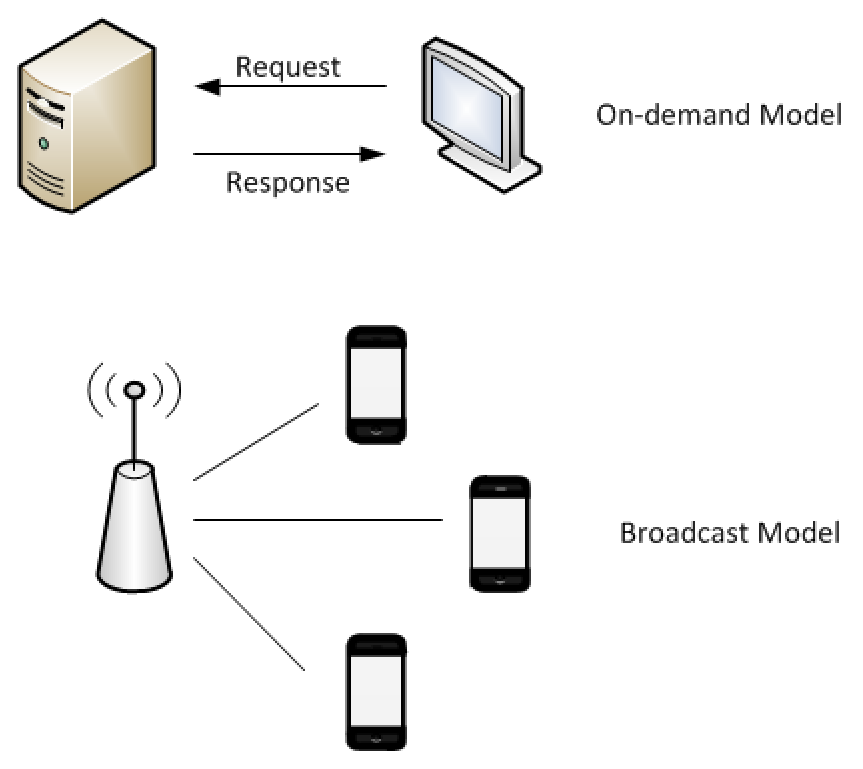
\includegraphics[width=2.5in]{Figures/on_demand.eps}
\caption{\small On demand and broadcast
models.\label{fig:broadcast}}
\end{center}
\end{figure}

A complete dissemination of all the records in the data set from
the server is a broadcast \emph{cycle}. A cycle follows another
cycle (see Figure~\ref{fig:bcast_cycle}). In this paper, we
sometime interchange cycle and program to denote the content of
the broadcast channel.

An inherit challenge of the broadcast model is the forward only
data model and that there is no random access of the data set.
When a client misses a piece of data from the current cycle, the
client must wait until the next cycle. The reverberations of these
properties of broadcast environment are: (1) we cannot adopt
disk-based skyline computation algorithms designed for traditional
database systems that require random access, and (2) we must
design a self-explanatory broadcast program using data index.

Many previous studies have done on different broadcast
environment. Multi-channels broadcast for data dissemination (and
techniques of data allocation) has been previously studied
\cite{DBLP:conf/cikm/HsuLC01} \cite{DBLP:conf/cikm/YeeN03}
\cite{DBLP:conf/mobicom/HameedV97}. Adaptive broadcast systems
that allow limited uplink (client to server) communication has
been studied in \cite{16350}. In this paper, we assume the
following properties for our broadcast environment:
\begin{enumerate}
\item Channel is forward-only. \item Only one channel is utilized.
\item No uplink bandwidth from clients to server.
\end{enumerate}

%The broadcast program is broken down into packets and each packet
%contains data records and each data record
%contains a number of fields (or attributes) as shown in
%Figure \ref{fig:bcast_cycle}. The entire broadcast program is considered
%a cycle. A new cycle is broadcasted after the cycle. Though the
%channel only broadcast one kind of data that is
%interesting to the clients, we assume that the data is different from one broadcast
%cycle to the next due to data updates between cycles. The consequence
%of different in data is that we cannot
%assume a records will broadcast at the same time in the next cycle and
%that the index structure could be vastly
%different between cycles.

\begin{figure}[h]
\begin{center}
\includegraphics[width=3.5in]{Figures/bcast_cycle.eps}
\caption{\small Broadcast program cycle}
\label{fig:bcast_cycle}
\end{center}
\end{figure}

Power consumption is a major concern since in this environment,
clients are small mobile devices, such as cellular phones, powered
by a small battery; therefore, power is an scarce and valuable
resource for these devices for most cases. Even for non-mobile
clients energy conservation is a desirable attribute for a system.
Actively listening to the broadcast channel is expensive in terms
of power usage. Most mobile devices is able to turn off the radio
receiver when it is not actively sending or receiving data to
conserve power.

To reduce the power consumption, an index is used to make the
broadcast cycle self-descriptive. As depicted in
Figure~\ref{fig:index_node}, An index provides additional
information in a broadcast program to tell the clients the
approximate time when a data records will be broadcasted. A
broadcast index is analogous to an index in traditional database
management systems in which the indexes provide the location of
data records and facilitate fast lookup of records. With the index
information, the clients can turn off the radio receiver and
transmitter to conserve power and only tune into the channel when
the desire data is being broadcasted.

%Similarly, wireless
%index tells the time when records will be broadcasted. With the index
%information, the clients can turn off the radio receiver and
%transmitter to conserve power and only tune into the channel when the
%desire data is being broadcasted. An example index would be for data
%in the range of [0, 10) will be broadcasted in time $t_1$, and for
%data in the range of [10, 20) will be broadcasted at time $t_2$ and so on
%as illustrated in Figure~\ref{fig:index_node}.

\begin{figure}[h]

\centering
\subfigure[2-D MBR]{
\includegraphics[width=1.4in]{Figures/mbr_2d.eps}
\label{fig:mbr_2d}
}
\subfigure[3-D MBR]{
\includegraphics[width=1.8in]{Figures/mbr_3d.eps}
\label{fig:mbr_2d}
}
\subfigure[]{
\includegraphics[width=1.8in]{Figures/index_node_entry.eps}
\label{fig:index_node_entry}
}
\caption{\small Tree Index.\label{fig:index_node}}
\end{figure}

%In this research, we study the way to embed data index in our
%broadcast program to provide efficient skyline query from broadcast
%program on air, while keeping the broadcast program useful to other
%applications. Our index technique is not overly specific as the index
%technique presented in \cite{Ha:2009:EEP:1616994.1617050} so that the
%broadcast program can only efficiently support skyline. In our
%technique we use generic, common tree index to be our index structure.
%Tree indexes are known to be generic and have been studied to support
%many other applications, for example range queries and k-nearest-neighbor
%($k$NN) queries. Since useful skyline queries involve multiple
%attributes, we utilize spatial indexes, such as R-Tree and R+-Tree,
%as our index structure although the data does not necessary contain
%spatial data in the sense of geo-spatial data. The relevant attributes
%forms a conceptual space in the spatial index. The reason we use spatial
%index so that multiple attributes can be indexed as shown in
%Figure~\ref{fig:skyline}. Existing wireless broadcast index techniques
%will be discussed in section \ref{sec:wireless_bcast_index}.

Adding index to a broadcast cycle also adds space overhead to the
cycle and ultimately consume more broadcast bandwidth. Quantities
that measure the efficiency of a wireless broadcast program are
defined below, of which \emph{tuning time} and \emph{access
latency} are well-known metrics and has been studied in other
works preceeding this paper \cite{dsi} \cite{data_on_air}
\cite{DBLP:journals/tmc/KuZW08} \cite{signature_and_caching}. We
also define \emph{Index Percentage} as a novel meansurement of the
space overhead of the index structure.

\begin{definition}[Index Percentage]\label{def:index_percentage}
The ratio of the space allocated to index to the space of the
entire cycle measure in bytes. This quantity is defined as $\rho =
\frac{\iota}{\omega}$.
\end{definition}

\begin{definition}[Initial Index Probe]\label{def:index_probe}
The amount of time for a client to get to the first index segment.
There are many methods of initial index probe, such as probing
every $\delta$ amount of time. Another method is to tune into the
channel the entire time until the first index is retrieved;
nonetheless this quantity is not added to the tuning time. This
quantity is denoted by $\alpha$.
\end{definition}

\begin{definition}[Tuning time]\label{def:tuning_time}
The total amount of time the client actively listening to the
channel in order to retrieve desire data. This is measured in
terms of the space of the index and data segments. This quantity
is denoted by $\beta$.
\end{definition}

\begin{definition}[Access latency]\label{def:access_latency}
The amount of time from when the client makes the request to when
the client receives all the desired data. Similar to tuning time,
this is also measured in terms of the space of the index and data
segments. This quantity is denoted by $\gamma$.
\end{definition}

%Skyline definition is definition~\ref{def:skyline},
%definition~\ref{def:index_percentage},
%definition~\ref{def:index_probe}
%By definition, the tuning time is directly proportional to the required energy consumption by the clients.
%Unfortunately, these two quantities are trade-offs for a broadcast program. When we try to reduce tuning
%time by including index, we increase the length of the program therefore increase access latency. If we
%do not include any index information, the program would be the shortest, but the client would have to listen
%to the entire program to get the desired data.


\section{Tree-based Distributed Index}\label{sec-index}

Before we present our skyline computation algorithm in the next
section, in this section how the index and data are allocated on
the broadcast channel to form the broadcast program. We introduce
depth-first distributed-index (DFDI), our index allocation
technique, that is based on the distributed index allocation
proposed in \cite{data_on_air}. The benefits of a distributed
index over other allocation methods has been discussed in section
\ref{sec:wireless_bcast_index}.

We utilize an R-Tree~\cite{DBLP:conf/sigmod/Guttman84} to index our
multi-dimensional data records. We assume that each node of an R-Tree
consists of $b$ number of entries, $\{E_1, E_2, ... E_b\}$, where
$b$ is the branching factor, or the number of children at each internal
node, of the index tree, as illustrated by Figure~\ref{fig:index_node}.
Each entry contains a pointer to a child index node, if the node is not
a leaf node, or a pointer to a set of data records, if the node is a leaf
node. The pointer is the time when the child item will appear on the
broadcast channel.

In addition, each entry contains an orthotope, or a $n$-dimensional minimal
bounding rectangle (MBR), that denote the extend of the child object pointed
by the pointer of the entry (see Figure~\ref{fig:index_node}). Each
rectangle $MBR$ is defined by two opposite corners, $MBR.min$ and $MBR.max$,
also known as the ``lower-left" and ``upper-right" corners of the rectangle.
$min = (min_1, min_2, ..., min_n)$ and $max = (max_1, max_2, ..., max_n)$
are $n$-dimensional points containing minimal and maximal value of each
attribute in the rectangle, respectively. In other words, $min_i$ is the
lower bound, and $max_i$ is the upper bound of $i$th attribute in $MBR$.

An advantage of using R-Tree is that
it is a flexible index that can support other spatial queries,
such as range queries and $k$NN queries.
Using an R-Tree also satisfies our goal of creating a flexible index that
supports combination of skyline queries.

\subsection{Broadcast Structure}

A broadcast program cycle is a linear representation of the index
tree and data and consists of \emph{index segments} and
\emph{data segments}. Index segments contains temporal pointers to
either another index segment or a data segment. Data segments
contain actual data records. Index and data segments intermingle
to for a broadcast program. Each index segment is further divided
into smaller units called buckets. Buckets are logical independent
units that represent a portion of the tree index. The purpose for
buckets is that a client does not have to download an entire index
segment if it only needs a bucket.

In addition to a list of temporal pointers, each index bucket also
contains a pointer to the next index segment and a pointer to the
beginning of next broadcast cycle. The purpose of these pointers
is to direct the client to the next index segment in the case that
the client tunes in at the index bucket but is not interested in
the data pointed by the index.

To save bandwidth, data segments do not contain any index
information other than data records. The broadcast program
structure is illustrated in Figure~\ref{fig:index_packet}.



%\subsection{Packet Format}
%A broadcast program consists of a series of packets. There are two types of packets that make
%up our program: data and index. The data packets carry the actual data records the clients are
%interested and the index packets contains the index of the data and when a record will be
%broadcasted in the cycle. The data and index packets intermingle to form the broadcast cycle.
%A series index packets is an index segment and a series data packets is a data segment as
%shown in Figure~\ref{fig:bcast_cycle} in section \ref{sec:wireless_broadcast}. The format
%in which the index and data packets are organized in a broadcast cycle is the
%broadcast structure.

%\begin{mydef}[Broadcast Structure] The format in which the index and
%    data packets are organized in a broadcast cycle.
%\end{mydef}

%In addition to pointing to a data segment, each index packet also has a pointer to the next
%index packet, $\tau_I$, and a pointer to the next broadcast cycle, $\tau_B$.
%The purpose of \emph{ind\_ptr} is to direct the client to the next index segment in the case that
%the client tunes in at the index packet but is not interested in the data pointed by the
%index. The purpose of the $\tau_B$ is to allow the client to retrieve the data from the
%beginning of a new broadcast cycle. Index packet structure is illustrated
%in Figure~\ref{fig:index_packet}. The attributes of an index packet is
%summarized in table~\ref{tab:index_attr}.

%\begin{equation}
%IndexPacket = ind\_ptr + bcast\_ptr + \{data\_ptr\}
%\end{equation}

\begin{figure}[h]
\begin{center}
\includegraphics[width=3.5in]{Figures/index_packet.eps}
\caption{\small Broadcast program cycle format with index segments
and data segments.}
\label{fig:index_packet}
\end{center}
\end{figure}

%\begin{table}[h]
%\centering
%\begin{tabular}{l|l}
%  \hline
%  {\bf Attribute}   &   {\bf Description}\\
%  \hline
%  %\emph{data\_ptr}  &   Pointer to data packet\\
%  \emph{ind\_ptr}   &   Pointer to next index packet\\
%  \emph{bcast\_ptr} &   Pointer to beginning of next broadcast\\
%  \hline
%\end{tabular}
%\caption{Index Packet Attributes}
%\label{tab:index_attr}
%\end{table}

%Imielinski, et al in \cite{data_on_air} also included \emph{ind\_ptr}
%and \emph{bcast\_ptr} in data packet. We do not include these attributes
%in data packets to save bandwidth at the cost the initial index probe.
%Consider that a client tunes into the channel at a data packet. The client
%will have to keep tuning into the channel until the next index packet to
%get a ``road map" of the program. On average, the client would have to
%listen to half of the data segment, \(\frac{ds}{2}\), to get to the next
%index packet. Consider that a pointer of time takes $ptr$ of broadcast
%bandwidth. Let $bf$ be branching factor of an index tree. If we include
%both pointers in each data packet, additional bandwidth to include the
%pointers would be $2 \times ptr \times (bf^h + 1)$.

%A data packet does not contain any pointer, but contains multiple data
%records. $DataPacket$ = Header + $P$ $\subseteq$ $T$, where P is a set
%of tuples, and T is a set of tuples that consists of the entire data set.

%\begin{figure}[h]
%\begin{center}
%\line(1,0){240}
%\begin{verbatim}
%... Header ...
%Data Record       Attribute       Attribute
%Data Record       Attribute       Attribute
%Data Record       Attribute       Attribute
%...
%\end{verbatim}
%\line(1,0){240}
%\caption{\small Data Packet Format.
%\label{fig:data_packet_format}}
%\end{center}
%\end{figure}

%\subsection{Index Packing}
%
%For many tree index structures, including R-Tree, the branching factor
%of each node depends on the application. For a large data set, the
%branching factor would be larger than a smaller data set, to reduce
%height for the index, but the space utilization for each node would
%be higher.
%
%The space requirement to pack an index node
%into a broadcast packet depends on the branching factor of the tree.
%The number of entries in an index node equals to the branching factor.
%For example, for an R-Tree with branching factor of 4, space is
%required to store 4 MBRs and pointers.
%Since every entry contains a MBR and a pointer, larger the
%branching factor, larger the space requirement per node. The relationship
%is defined as follows:
%
%\begin{equation}
%s_n = b \times (s_{ptr} + s_b)
%\end{equation}
%
%Each index node can be packed into one index packet when the number of
%index entry is large. In this case the space utilization of each node
%before index replication is the space per node plus space of two
%pointers to the next index segment and broadcast cycle times the number
%of nodes in the index.
%
%\begin{equation}
%s_i = (b^{h} + 1) \times (s_n + 2 \times s_{ptr})
%\end{equation}
%
%If we pack multiple index nodes into one index packet, we can reduce
%the number of index pointers. In this case, if the next
%index node is in the same packet, we keep the same space utilization
%of a pointer but signify that the pointer to the next node is not a
%temporal, but instead a storage location within in this packet. The
%space utilization in this case is
%
%\begin{equation}
%s_i = \frac{b^{h} + 1}{n_p} \times (s_n + 2 \times s_{ptr})
%\end{equation}
%
%
%\begin{table}[h]
%\centering
%\begin{tabular}{c|l}
%  \hline
%  {\bf Notation} & {\bf Description}\\
%  \hline
%  $b$ & Branching factor of index tree.\\
%  $h$ & Height of index tree.\\
%  $s_{ptr}$ & Space utilization per pointer (ex: 16 bits).\\
%  $s_n$ & Space utilization per node.\\
%  $s_b$ & Space utilization per MBR.\\
%  $s_i$ & Total space of index tree.\\
%  $n_p$ & Nodes per packet.\\
%  \hline
%\end{tabular}
%\caption{Notations of packet format.}
%\label{tab:pf_notations}
%\end{table}

%\subsection{Motivation for DFDI}
%Consider that we have an R-Tree to index our multi-dimensional data, we
%need to consider the broadcast structure and format so that the index
%and data packets can be broadcasted on the same channel. Tree index
%structures are of particular interest since trees are non-linear whereas
%broadcast program is strictly linear. We consider two techiniques of
%embedding index as motivation for our index technique.
%
%One method is to embed the entire
%index tree at the beginning of the broadcast program as one big index
%segment (one huge packet or a series of continuous index packets). A
%drawback of this approach is that if the client misses the index segment,
%then no further processing can be done with the current cycle and the
%client has to wait for the next cycle. Another drawback is that the client
%have to download the entire index, although, the client may only be
%interested in a portion of the data. In addition, with our approach
%that the data packets do not have pointer to the next broadcast cycle or
%the next index segment, the client would not have a way to find out the
%time for the next cycle, except for continuously listening until the
%next cycle begins with new index.
%
%To mitigate the drawback, we could replicate and place the entire index
%segment of the previous method through out the broadcast program as
%proposed and discussed in \cite{data_on_air}. The drawback is that
%replicating the complete index several times increases
%the size of the broadcast program. For large data sets with large number
%of index nodes, this is inefficient.
%
%$\rightsquigarrow$ Consider an example that each pointer in an index packet is 16-bit
%(2 bytes). All 3 pointers takes 6 bytes.
%
%When coming in the middle of the program, a client really need an index
%packet, not the entire index, as a road map to when the next index
%will be available. This is the idea of the distributed index, in which
%the index is distributed in the program, but only a portion of the
%index is replicated.

\subsection{DFDI Allocation}

We have data indexed by a R-Tree. Our task now is to publish both
data and index on to the linear broadcast channel. DFDI allocates
space for index and data by performing a depth-first traversal of
the index tree as illustrated in Figure~\ref{fig:index_struct}. In
this process, the root index node $A$ is first included in the
cycle because it is first traversed. Index node $B_1$ is then
included in the program followed by $C_1$, then the data items
$D_1$ and $D_2$. One might argue that why use depth-first
traversal of the index tree, instead of breadth-first traversal
(BFT). The reason is that BFT would cluster all index into one
enormous index segment at the beginning of a cycle and basically
create a 1-time index.

DFDI replicate $L_r$ levels of the index tree $b$ times, where the
root node is considered level 1. Replication helps the clients get
a broader picture of upcoming broadcast items. When an index node
is replicated, only the MBRs that have no been broadcasted is
published; therefore the replication is \emph{not a complete
replication} of the node. Given $N$ to be the current node to be
published, if the level of $N$ is $L_r + 1$ or less, then the
parent of $N$ is replicated. Otherwise the parent is not
replicated.

An example is shown in Figure~\ref{fig:index_struct}, the root and
the B level index nodes are replicated. The replication helps the
client gets a broader picture of upcoming broadcast item. Of
course the best view would be to replicate the entire index, but
this would be the complete replication as discussed before and we
try to avoid to save broadcast bandwidth.
%Given two sibling index nodes $A$ and
%$B$ and their parent index node $P$, the following rules determine if
%an index node is replicated in the broadcast program:
%
%\begin{enumerate}
%\item If $A$ is the current index, and $P$ is part of the replicated
%        portion of the index, then $A.ind\_ptr$ points to an index packet
%        and segment that contains both $P$ and $B$.
%\item If $A$ is the current index, and $P$ is \emph{not} part of the
%        replicated portion of the index, then $A.ind\_ptr$ points to
%        an index packet (or segment) that contains only $B$.
%\end{enumerate}

\begin{figure}[h]
\begin{center}
\includegraphics[width=3.5in]{Figures/bcast_struct.eps}
\caption{\small Index Structure. \label{fig:index_struct}}
\end{center}
\end{figure}

\begin{algorithm}
\algsetup{linenosize=\small,linenodelimiter=. }
\caption{DFDIPublish($Node$, $Level$, $L_r$)}
\label{alg:DFDIPublish}
\begin{algorithmic}[1]

\STATE PushToChannel($Node$) \COMMENT{Assume temporal ptrs are
known} \IF{$Node$ is Leaf}
    \FORALL{DataSegment in $Node$}
        \STATE PushToChannel(DataSegment)
    \ENDFOR
\ELSE
    \FORALL{ChildNode in $Node$}
        \STATE DFDIPublish(ChildNode, $Level$++)
        \IF{$L_r$ $\leq$ $L$ AND NOT Last ChildNode}
            \STATE PushToChannel($Node$)
            \COMMENT{Replication}
        \ENDIF
    \ENDFOR
\ENDIF
\end{algorithmic}
\end{algorithm}
%The space saving

%\subsection{Broadcast Structure}

%In this solution R-Tree is used to index data records. The records are presented geometrically in
%the R-Tree index as illustrated in Figure \ref{fig:skyline_mbr}, which shows the R-Tree representation of the records
%of Figure \ref{fig:data_records}. The R-Tree is not necessary used to index spatial data. Note that
%the reason R-Tree is used is because of its multi-dimension index capability and that we are able
%to multiplex multiple attributes in the same index. Almost
%any spatial index that supports space indexing will work with our approach. We choose R-Tree because its popularity
%nd support for high-dimensional data.

%As shown in Figure \ref{fig:skyline_mbr},  each axis of the Euclidean space represents a dimension
%(or attribute) in the dataset. For example, the x-axis represents the distance of the hotels from the beach
%and y-axis represents the price of the hotels. The records are inserted into an R-Tree as presented Figure \ref{fig:skyline_mbr}.

%\begin{figure}
%   \centering
%   \subfloat[Data records]{\label{fig:tablel}\includegraphics[width=1.5in]{table.eps}}
%   \subfloat[Data records inserted into R-Tree]{\label{fig:skyline_mbr}\includegraphics[width=1.5 in]{rtree_pr.eps}}
%   \caption{Data and R-Tree Index}
%   \label{fig:data_skyline_mbr}
%\end{figure}

%\begin{figure}[h]
%\begin{center}
%\includegraphics[width=2in]{Figures/table-eps-converted-to.pdf}
%\caption{\small Data Records.\label{fig:data_records}}
%\end{center}
%\end{figure}

%\begin{figure}[h]
%\begin{center}
%\includegraphics[width=3in]{Figures/rtree.pdf}
%\caption{\small Data Records inserted into R-Tree.\label{fig:skyline_mbr}}
%\end{center}
%\end{figure}

%The R-Tree index is multiplexed with the data records in the broadcast program using the distributed index technique as
%discussed in section \ref{sec:wireless_bcast_index} since the technique offers one of the best
%trade-off between broadcast space utilization and probing time for the client to find the first index packet.
%The broadcast program contains the intermingle of data packets and index packets as shown in Figure \ref{fig:bcast_cycle}.

%The index technique replicates upper levels of the index tree and does not
%replicate the lower portion (close to the leaves) of the index. The reason for only replicate a
%portion of the index is to conserve broadcast bandwidth while maintain the ability for the clients
%to recognize the state of the broadcast without waiting for the next cycle. The %replicated portion
%is broadcasted periodically, while non-replicated portion only broadcasted near the data item.

%The index packets are distributed amount the broadcast program, as in (1, m) index. The packets that contain replicated
%portion of the R-Tree index points to (the time of) the packets that contain non-replicated index. Similarly, the packets
%that contains non-replicated portion of the index eventually points to the data records. When we say point, or pointer,
%we mean an item, $p$, has the time of broadcast of another item $c$, denoted $p \to c$. See Figure \ref{fig:index_struct}.

\subsection{Analysis}

This section presents the efficiency analysis of our index design.
The efficiency metrics are defined in section 2.2.

\subsubsection{Index Percentage}

Index percentage measures the space overhead of the index
structure. It is defined to be the ratio between the space
allocated to index on the broadcast cycle to the length of the
entire broadcast cycle.

Let $L_r$ be the levels of replication (for example, $L_r$ for
Figure~\ref{fig:index_struct} is 2), $\eta$ be the space required
for an index node, and $\varepsilon$ be the space required for an
index node entry. The number of nodes replicated in the cycle is
$\displaystyle\sum\limits_{i=0}^{L_r-1} b^i$. For each replicated
node, the replication does not replicate the entire index node,
only the MBRs that has not been pushed to the channel; therefore,
additional space for each replicated node is
$\eta\displaystyle\sum\limits_{i=1}^{b-1} \frac{i}{b}$ or
$\varepsilon\displaystyle\sum\limits_{i=1}^{b-1} i$. The total
space taken by index is the space for each node, plus the
additional space for each replicated node and it is given by:

\begin{equation}
\iota = \eta(\displaystyle\sum\limits_{i=0}^{L_r-1} b^i
\displaystyle\sum\limits_{i=1}^{b-1} \frac{i}{b} +
\displaystyle\sum\limits_{i=0}^h b^h)
\end{equation}

Let $\theta$ be the size of the entire data set. The length of the
broadcast cycle is the space of the index plus the space of the
data:

\begin{equation}
\omega = \eta(\displaystyle\sum\limits_{i=0}^{L_r-1} b^i
\displaystyle\sum\limits_{i=1}^{b-1} \frac{i}{b} +
\displaystyle\sum\limits_{i=0}^h b^h) + \theta
\end{equation}

\subsubsection{Initial Index Prob}

The distributed index divides the entire data set into smaller
data segments and reduces the initial prob of first index segment.
The length of each data segment, denoted by $\varsigma$, is
determined by the number of index segments distributed among the
broadcast cycle. As one see from Figure~\ref{fig:index_struct},
there are four leaf-nodes and the data is divided into four
segments; therefore, the number of data segment is $b^h$ and size
per data segment is

\begin{equation}
\varsigma = \frac{\theta}{b^h}
\end{equation}

If we consider that the prob time is 0 when a client tunes in at
an index segment, then the expected initial index prob is the
average of length of each data segment:

\begin{equation}
E(\alpha) = \frac{2\theta}{b^h} = \frac{2\theta}{m}
\end{equation}

This is a big time reduction compare with one-time index prob.


\section{Pruning Region Broadcast Skyline}\label{sec-pruning}

In this section, we present our point-based-pruning and index-based-pruning
skyline computation algorithms. Point-based-pruning strategy is
our first attempt to formulate a pruning-based algorithm and guarantees
correct result with or without a broadcast index.
%useful
%when MBRs of the index do intersect as in typical R-Tree structure.
Index-based-pruning generally provides better performance by performing
early pruning. We present two index-pruning strategies here.
%but requires that the MBRs of index do \emph{not} intersect.
The algorithms utilize the R-Tree index and allocation
method described in previous section to build a pruning region to
eliminate unwanted data records. Point-based-pruning skyline algorithm
is explained and followed by index-based-pruning algorithm.
%In addition, to simplify our demonstration, we
%first consider 2-dimensional skyline. Later we show how our
%approach can be easily extended to higher dimensions.

%Since a pruning region is the core of solution, we defined it
%here.

\begin{definition}[Pruning Region]
%A region in the space
%$R = D_1 \times D_2 \times ... \times D_n$ that is dominated by
%a subset of $P$ that has been examined so far.
Given the data space defined by $D_1 \times D_2 \times ... \times D_n$,
where $D_i$ is the data domain of attribute $i$,
a pruning region is a pair of a pivot point and an ordered list of
preference specifiers $(p, \sigma)$ that specifies a region of the data
space that has been dominated by a subset of the data-set. As
defined in Section~\ref{sec-prelim}, $\sigma_i$ is one of the values in
$\{min, max\}$.
\end{definition}

A pivot point, denoted by $p$ here, is a n-dimensional point in the
n-dimensional data space that defines the bounds of a pruning region.
The bounds is defined by the list of preference specifiers. For each
attribute $i$, if $\sigma_i = min$, then $p_i$ is the lower bound
of the pruning region for $i$th dimension and the region extends to
the maximal value for $i$th dimension. Similarly, if $\sigma_i = min$,
then $p_i$ is the lower bound and extends to minimal value of data
dimension. Pivot point and pruning region is illustrated in
Figure~\ref{fig:rtree_pr_2d} and \ref{fig:rtree_pr_3d}. Pruning regions
are illustrated as the gray regions and bounded by pivot points $b$ and
$d$. As illustrated, a pruning region is a region of n-dimensional
space (or a n-dimensional box) that has been dominated by $p$ and can be
ignored in the upcoming broadcast data stream.

\begin{corollary}\label{co:pivot_point}
The pivot point of a rectangle dominates all points of the rectangle.
\end{corollary}

\begin{proof}
Given a pivot point, $p$, of a rectangle, $r$, for all attribute $i$,
if $\sigma_i = min$ then $p_i = r.min_i$, if $\sigma_i = max$ then
$p_i = r.max_i$. This implies that the pivot point has the best value
for all attributes in the rectangle, therefore no points can dominate it
and it dominates all points of the rectangle except for itself.
\end{proof}

\begin{figure}[!h]
\label{fig:rtree_pr}
\centering
\subfigure[2-D with preference specifiers (min, min)]{
\includegraphics[width=1.6in]{Figures/rtree_pr2.eps}
\label{fig:rtree_pr_2d}
}
\subfigure[3-D with preference specifiers (min, min, max)]{
\includegraphics[width=1.6in]{Figures/rtree_pr_3d.eps}
\label{fig:rtree_pr_3d}
}
\caption{Pruning region with pivot points b and d}
\end{figure}


\subsection{Point-Based Skyline Pruning}

To compute the skyline, a pruning region is progressively
augmented as more data records are examined. The algorithm keeps
track of a list of candidate skyline points, $S$, and a pruning
region that is the union of pruning region of $S$. As the pruning
region grows, any $p$ in $S$ that is inside the pruning region is
removed and any new MBR received from the broadcast cycle that is
inside the pruning region is ignored. At the end of the algorithm,
points in $S$ that are not removed are returned as skyline.

Skyline computation is illustrated in
Algorithm~\ref{alg:PBSkyline}. At the beginning of the algorithm,
the client does not have any candidate skyline points; therefore,
the pruning region, $R$, is null ($R =$ {\o}).
In this state, the client cannot prune any R-Tree MBR and
therefore must stay tuned into the channel for the first index bucket
broadcasted on the channel. The client follows a series of index
buckets to the first data segment.
When a data segment is reached, the client does:
\begin{enumerate}
\item Download all data points from the data segment.
\item Compute skyline points, $S_0$, using any existing skyline algorithm
        (NL, BNL, NN, BBS).
\item For each point in $S_0$, compute a pruning region, $R'$, and and remove
    all points in $S$ covered by $R'$.
\item For each $R'$, $R = R \cup R'$
\item Add each point in $S_0$ to $S$.
\end{enumerate}
This repeats until the entire space is inside the pruning region.

Note that the points found in each data segment are only candidate skyline
points since there could data broadcasted later
that dominate the earlier candidate points. If a candidate point
$p_2$ dominates earlier point $p_1$, then $p_1$ is removed from
$S$ and the pruning region is enlarged by the later point $p_2$.
%Algorithm~\ref{alg:PBSkyline} ends when there is no more MBR in
%the broadcast cycle that is outside the pruning region.

ComputePruneRegion() in Algorithm~\ref{alg:PBSkyline} is described
next.
%Note that Algorithm~\ref{alg:PBSkyline} utilizes
%ComputePruneRegion(), which is listed in
%Algorithm~\ref{alg:ComputePruneRegion1}. ComputePruneRegion in
%Algorithm~\ref{alg:ComputePruneRegion1} computes a pruning region
%from a list of candidate skylines points, $S$, based on the
%preference specifiers, $\sigma$. The algorithm loops through each
%point, $s$ in the list, $S$, computes the pruning region for $s$
%and union to the final pruning region. The algorithm returns the
%total pruning region after all points are processed.

\begin{algorithm}
\algsetup{linenosize=\small,linenodelimiter=. }
\caption{Point-Based Skyline($\sigma$)} \label{alg:PBSkyline}
\begin{algorithmic}[1]

\STATE $S \gets$ \o
\STATE $R \gets$ \o
\STATE $index \gets$ search first index bucket
\STATE $queue.enqueue(index.pairs(mbr, time))$
\WHILE{$queue$ is not empty}
    \STATE $bucket \gets GetBucket(queue.dequeue)$
    \IF{$bucket$ is index bucket}
        \FORALL{$pair(mbr, time)$ in $bucket$}
            \IF{$pair$ is not in $pruneRegion$}
                \STATE $queue.enqueue(pair)$
            \ENDIF
        \ENDFOR
    \ELSE
        \STATE $S_0 \gets ComputeSkyline(bucket, \sigma)$
        \STATE $R' \gets ComputePruneRegion(S_0, \sigma)$
        \STATE $Prune(S, R')$
        \STATE $Prune(queue, R')$
        \STATE $R \gets R \cup R'$
        \STATE $S \gets S \cup S_0$
    \ENDIF
\ENDWHILE \RETURN $S$
\end{algorithmic}
\end{algorithm}

%\begin{algorithm}
%\algsetup{linenosize=\small,linenodelimiter=. }
%\caption{ComputePruneRegion($S$, $\sigma$)}
%\label{alg:ComputePruneRegion1}
%\begin{algorithmic}[1]
%
%\STATE $totalR \gets$ \o \FORALL{$p$ in $S$}
%    \STATE $tempR \gets$ ($-\infty$ to $\infty$) for all dimensions
%    \FOR{$i = 0$ to $n$}
%        \IF{$\sigma[i] = MIN$}
%            \STATE $tempR \gets tempR \bigcap (\infty \bigcup ... \bigcup (s[i]~to~\infty)_i \bigcup ... \bigcup \infty $)
%        \ELSE
%            \STATE $tempR \gets tempR \bigcap (\infty \bigcup ... \bigcup (min(D_i)~to~s[i])_i \bigcup ... \bigcup \infty $)
%        \ENDIF
%    \ENDFOR
%    \STATE $totalR \gets totalR \bigcup tempR$
%\ENDFOR \RETURN $totalR$
%\end{algorithmic}
%\end{algorithm}

\subsubsection{Pruning and Pruning Region}
Here we describe pruning region computation and pruning strategy listed in
Algorithm~\ref{alg:PBSkyline}.

%The formulation of a pruning region depends on a pivot point, here we denote
%it with $p$, and the preference specifiers
%of the attributes of the data. For each axis (attribute) of the data space,
%the preference could be either MIN or MAX. For an axis $i$ with MIN specifier,
%the pruning space is from $p.i$ to $\infty$ (or maximum value for the attribute).
%Similarly, for the axis with MAX specifier, the pruning space is from $p.i$ to
%$-\infty$ or minimum value of the attribute. For data of positive value, the
%minimum value would be 0.

To determine if a point $q$ is covered (should be pruned) by a pruning
region, all attributes of the point has to be checked against the pivot
$p$ of the pruning region. The condition for a point to be covered is that
all attributes of point $q$ is inside the pruning region. For a point to
be covered, each attribute $i$ satisfy one of the following:
\begin{enumerate}
  \item If $\sigma_i$ = MIN, then $q_i \geq p_i$.
  \item If $\sigma_i$ = MAX, then $q_i \leq p_i$.
\end{enumerate}

To determine if an index bucket is covered by a pruning region and should be
ignored when computing skyline as in Point-Based Skyline discussed previously,
we need to determine if the MBR of the index bucket is covered. To do so, we
need to determine the pivot point of the MBR according to the preference
specifiers. Based on Corollary~\ref{co:pivot_point}, if the pivot
point of a pruning region dominates the pivot point of the MBR, then the
index bucket can be pruned and ignored, since the pivot point of the MBR
dominates the entire bucket.
Following the definition of a rectangle defined in
Section~\ref{sec:wireless_broadcast},
a MBR is covered by a pruning region if its pivot is covered by the pruning
region as illustrated by Figure~\ref{fig:pruning}. A pruning region is
illustrated in gray and
defined by pivot point $p$ with the skyline query specifiers of
$(X = min, Y = max)$. MBR $A$ can be pruned since its pivot $p_1$ falls
inside the pruning region, while although MBR $B$ is partially covered by
the pruning region, it can not be pruned since its pivot, $p_2$, does
not fall inside the pruning region, in other words $p$ dominates $p_1$, but
does not dominate $p_2$.

\begin{figure}[h]
\begin{center}

\includegraphics[width=2.5in]{Figures/pruning.eps}
\caption{\small Pruning region defined by $p$ and preference specifier
$(X = min, Y = max)$ and MBRs A and B.}
\label{fig:pruning}
\end{center}
\end{figure}

%\subsubsection{MIN and MAX Attributes}
%In two dimensional skyline when we consider both MIN and MAX
%skyline specifier, there are totally four possibilities. Let x,
%and y be the two attributes of interest, the four possible skyline
%queries we can make out of the two attributes are (MIN $x$, MIN
%$y$), (MIN $x$, MAX $y$), (MAX $x$, MIN $y$), and (MAX $x$, MAX
%$y$). Similar to the (Min $x$, and Min $y$) case, the algorithm
%progressively builds pruning region from the minimal bounding box
%of the index tree and data points received from the broadcast
%program.

%The pruning region orientation differs slightly for each case.
%Given a candidate skyline point $p$, the pruning region for an MIN
%attribute, $x$, would span from $p.x$ to positive infinity. In
%other words the range of the pruning region for the attribute
%%attribute would have pruning region span from 0, to $p.x$, [0,
%$p.x$], for data that does not include negative values or from
%negative infinity to $p.x$, ($-\infty$, $p.x$], for data that
%contains negative values.

%\begin{figure}[ht]
%\centering

%\subfigure[Subfigure 1 caption]{
%   \includegraphics[width=0.5in] {skyline_minx_miny.pdf}
%   \label{fig:subfig1}
% }

% \subfigure[Subfigure 2 caption]{
%   \includegraphics[width=0.5in] {skyline_minx_maxy.pdf}
%   \label{fig:subfig2}
% }

% \subfigure[Subfigure 3 caption]{
 %  \includegraphics[scale=0.5] {skyline_maxx_maxy.pdf}
   %\label{fig:subfig3}
% }


%\label{myfigure}
%\caption{Global figure caption}
%\end{figure}

\begin{comment}
\begin{figure}[h]
\begin{center}
\includegraphics[width=2.5in]{Figures/skyline_minx_miny.pdf}
\caption{\small MIN $x$, MIN $y$ and pruning region.
\label{fig:skyline_minx_miny}}
\end{center}
\end{figure}

\begin{figure}[h]
\begin{center}
\includegraphics[width=2.5in]{Figures/skyline_minx_maxy.pdf}
\caption{\small MIN $x$, MAX $y$ and pruning region.
\label{fig:skyline_maxx_maxy}}
\end{center}
\end{figure}

\begin{figure}[h]
\begin{center}
\includegraphics[width=2.5in]{Figures/skyline_maxx_miny.pdf}
\caption{\small MAX $x$, MIN $y$ and pruning region.
\label{fig:skyline_maxx_maxy}}
\end{center}
\end{figure}

\begin{figure}[h]
\begin{center}
\includegraphics[width=2.5in]{Figures/skyline_maxx_maxy.pdf}
\caption{\small MAX $x$, MAX $y$ and pruning region.
\label{fig:skyline_maxx_maxy}}
\end{center}
\end{figure}
\end{comment}


\subsection{Index-Based Skyline Pruning}

The drawback of Algorithm~\ref{alg:PBSkyline} is that the
pruning regions are formed from candidate skyline points that have
been retrieved from the broadcast channel. The pruning regions are
formed late in the program since data segments are broadcasted
after corresponding index segments.
%The reason we only use data
%records as criteria to form pruning region to accommodate
%overlapping region in index tree (such as in R-Tree).
In this section we present index-based pruning algorithm that perform
early index-based pruning and two pruning strategies that produce
the same tuning time from a client view.
The expectation is that with early pruning,
more of the index tree would be pruning and improve efficiency over
point-based pruning strategy.
%One of index structure that supports non-overlapping index regions is
%R+-Tree which can be found in ~\cite{DBLP:conf/vldb/SellisRF87}.

The two index-pruning strategies are one-region and n-regions. 
The one-region pruning strategy, forms only one pruning region per
MBR of the index tree as illustrated by Figure~\ref{fig:ibp_a}.
This strategy is based on the claim that we can prune everything from
the pivot point of the MBR of the index. The following present a short
proof of the correctness of this claim for a 2-dimensional case:

\begin{proof}
Given a 2-dimensional MBR, $r$, and skyline query of $(min, min)$.
There must exist at least one point, $p$,
in $r$ such that $p_2 = r.min_2$, $p_1$ in range
$[r.min_1, r.max_1]$. Similarly, there must exist another
point, $q$ such that $q_1 = r.min_1$, $q_2$ in range
$[r.min_2, r.max_2]$.

$p$ dominates anything to the right of $p_1$ and above
$r.min_2$ and $q$ dominates all records above $q_2$ and to
the right of $r.min_2$. We extend the $p_2$ value of the prune
region of $p$ and the $q_1$ value of the pruning region of $q$
and these two are the same as the values for the pruning region of
point $(r.min_1, r.min_2)$. Since MBRs do not overlap, pruning
regions for point $(r.min_1, b.min_2)$ is the pruning region
of the MBR $r$.
\end{proof}
Although this approach is simple, the client must keep track of the
current MBR which is inside the pruning region, but should not be
pruned. For example, MBR $A$ is inside pruning region, but it is the
MBR of the index currently being investigated. The region of $A$
should not be pruned.


n-region pruning strategy is illustrated in Figure~\ref{fig:ibp_b}.
This pruning strategy is more natural way of query evaluation. The
remaining of this section discuss the point-based skyline evaluation
algorithm using n-region strategy.

Index-Based skyline algorithm start the same way as the point-based
skyline algorithm in that initially, the pruning region is null and
the client must stay tuned to the broadcast channel until it finds
the first index bucket. When the client receives an index bucket that
is not covered by the pruning region (in this case it is the first
index bucket), it performs the following:
\begin{enumerate}
\item For each entry, create a set of $n$ pruning regions, $R'$,
    where $n$ is the dimensionality of the dataset. This is explained
    below.
\item Remove points in candidate skyline, $S$, that are covered by
    $R'$.
\item Add the new pruning regions, $R'$, to the total pruning region.
    For each $R'$, $R = R \cup R'$.
\end{enumerate}
The rationale for step 1 above to create $n$ pruning regions for each
entry is that we want prune the data dominated by the entry, but we
do not want to prune the data that is bounded by the MBR of the entry
before we download data. Figure~\ref{fig:ibp}
demonstrates this idea. Assuming the current index bucket we get from the
broadcast channel is MBR A and it is not covered by the pruning region
$R$, since MBR A is not covered, we want to follow this index to its
children $A_1$ and $A_2$ and ultimately download the data points in $A$. If we
form the pruning region of A using the strategy of Figure~\ref{fig:ibp_a},
then $A_1$ and $A_2$ will be pruned before we have the chance to download the
data. Following, the strategy of Figure~\ref{fig:ibp_b}, we have a chance
to download the data.

\begin{figure}
  \centering
  \subfigure[Pruning with one Pruning Region]{
    \label{fig:ibp_a}
    %\begin{minipage}[h!]{0.5\textwidth}
      \includegraphics[width=1.5in]{Figures/index_based_pruning_a.eps}
    %\end{minipage}
    }
  \subfigure[Prune with $n$ Pruning Regions]{
    \label{fig:ibp_b}
    %\begin{minipage}[h!]{0.5\textwidth}
      \includegraphics[width=1.5in]{Figures/index_based_pruning_b.eps}
    %\end{minipage}
    }
  \caption{Index-Based Pruning Strategies (min, min)}
  \label{fig:ibp}
\end{figure}

To create $n$ pruning regions, we need a pivot point for each pruning
region. Let $r$ be an orthotope (a MBR) and $i, j = \{1, 2, ... n\}$, such
that $p_i$ is the $i$th pivot point of $r$, and $p_{i,j}$ is the $j$th
attribute (or coordinate) of $i$th pivot point. $p_i$ is computed in the
way that $p_{i,i}$ is the opposite of $\sigma_i$ and $p_{i,j}$ is the same
as $\sigma_i$ for all $j \neq i$.

For example, for a skyline query of all MIN attributes,
$\sigma = (MIN, MIN, MIN)$ and therefore $\sigma_i = MIN$. In this case,
$p_{i,i} = r.max_i$ and $p_{i,j} = r.min_j$ for $j \neq i$.

\begin{algorithm}
\algsetup{linenosize=\small,linenodelimiter=. }
\caption{Index-Based Skyline($\sigma$)} \label{alg:IBSkyline}
\begin{algorithmic}[1]

\STATE $S \gets$ \o
\STATE $R \gets$ \o
\STATE $index \gets$ search first index segment
\STATE $queue.enqueue(index.pairs(mbr, time))$
\WHILE{$queue$ is not empty}
    \STATE $bucket \gets GetBucket(queue.dequeue)$
    \IF{$bucket$ is Index Packet}
        \FORALL{$entry \gets pair(mbr, time)$ in $bucket$}
            \IF{$R$ is not in $entry$}
                \STATE $queue.enqueue(pair)$
                \STATE $R' \gets ComputePruneRegion(e.mbr, \sigma)$
                \STATE $Prune(S, R')$
                \STATE $Prune(queue, R')$
                \STATE $R \gets R \cup R'$
            \ENDIF
        \ENDFOR
    \ELSE
        \STATE $S \gets S \cup ComputeSkyline(bucket)$
    \ENDIF
\ENDWHILE \RETURN $S$
\end{algorithmic}
\end{algorithm}

%\begin{algorithm}
%\algsetup{linenosize=\small,linenodelimiter=. }
%\caption{ComputePruneRegion($B$, $\sigma$)}
%\label{alg:ComputePruneRegion2}
%\begin{algorithmic}[1]
%\STATE $R \gets$ \o \FOR{$i = 0$ to $n$}
%    \IF{$\sigma[i] = MIN$}
%        \STATE Add dimension $i$ to $R$ from 0 to $\infty$
%    \ELSE
%        \STATE Add dimension $i$ to $R$ from 0 to $B.i_{max}$
%    \ENDIF
%\ENDFOR \RETURN $R$
%\end{algorithmic}
%\end{algorithm}

%\subsubsection{Data Preparation}
%The data and index preparation is the same as in Solution1. The only difference is that instead
%of indexing the data with R-Tree, this solution index the data with R+-Tree. The attractiveness of
%this index structure is non-overlapping MBR and we can quickly find the pruning region in our
%algorithm. Give an example of why overlapping would cause a problem.

%A drawback of this index technique is creating an R-Tree without overlapping MBRs incur
%computational overhead (cite).

\begin{comment}
\begin{figure}[h]
\begin{center}
\includegraphics[width=2in]{Figures/R+Tree-eps-converted-to.pdf}
\caption{\small R+-Tree Index.\label{r+tree}}
\end{center}
\end{figure}
\end{comment}

%\subsubsection{Skyline Computation}
%
%We start with pruning region that covers space. As soon as our algorithm receives the first index
%segment we get a sense of the data distribution in space we can start forming pruning regions.
%Consider example [provide example and attach figure].  The entire index tree consists of MBRs
%A and B. Let $Min(MBR)$ be the corner of MBR that has minimum of all dimension and $Max(MBR)$
%be the corner that has maximum of all dimension. Since $Min(B)$ < $Min(A)$, we can immediately
%form the pruning region, and prune MBR A.

%Note, we don't need to consider sub-MBRs inside A and B. Since the MBRs do not overlap, the
%entire region cover by A is dominated by B. Comparing with Solution 1, we don't have to traverse
%the tree to the leaf nodes to start forming pruning regions; instead, we can obtain pruning regions
%as early as the root node of the index. This has improvement in tuning time.

%Consider all possibilities.

%\subsubsection{Correctness Verification}

%We consider the correctness of this algorithm for the MIN $x$, MIN
%$y$ case. This verification can be easily applied to other cases
%with combinations of attribute specifiers. Our goal is to prove
%the correctness of our index-based pruning algorithm. We want to
%show that we can form pruning regions from the MBR of an index
%node instead of wait until we receive data records as in
%Algorithm~\ref{alg:PBSkyline}. We also want to show that this
%algorithm does not prune false negatives (more than it should
%prune).
%
%We can form pruning region from the MBR of the index because the
%MBR of R+-Tree does not overlap. As we mentioned earlier in this
%paper, this technique does not work for index structures that
%allow overlapping index regions such as R-Tree and R*-Tree
%\cite{Beckmann:1990:RER:93597.98741}.
%
%Given a MBR, $b$, of data index that encloses data records, the
%$b$ is bounded by two points $(x_{min}, y_{min})$, $(x_{max},
%y_{max})$ and these points denote the lower-left and upper-right
%corners of the MBR respectively. There must exist a point, $p_1$,
%in $b$ such that $p_1.y = b.y_{min}$, $p_1.x$ in range
%$[b.x_{min}, b.x_{max}]$. Similarly, there must exist another
%point, $p_2$ such that $p_2.x = b.x_{min}$, $p_2.y$ in range
%$[b.y_{min}, b.y_{max}]$.
%
%$p_1$ dominates anything to the right of $p_1.x$ and above
%$b.y_{min}$ and $p_2$ dominates all records above $p_2.y$ and to
%the right of $b.x_{min}$. We extend the $y$ value of the prune
%region of $p_1$ and the $x$ value of the pruning region of $p_2$
%and these two are the same as the values for the pruning region of
%point $(b.x_{min}, b.y_{min})$. Since MBRs do not overlap, pruning
%regions for point $(b.x_{min}, b.y_{min})$ is the pruning region
%of the MBR $b$.

%\subsection{Skyline of Higher-Dimension}
%For skyline queries that involves more than two query attributes,
%we need to consider computation of skyline of higher dimension.
%Due to the generic nature of our algorithm, we can extend our
%algorithm to higher dimensions.
%
%Similar to skyline in two-dimension, we first need to index our
%data in an index structure. R-Tree and other spatial index
%structure, such as KD-Tree, can support data of arbitrary
%dimension. KD-Tree and Quad-Tree are better choice here due to
%lower computation complexity of building the index for
%higher-dimensional data. %We build our index as illustrated in Figure \ref{fig:rtree3d}.

%\begin{figure}[h]
%\begin{center}
%\includegraphics[width=3in]{Figures/rtree3d-eps-converted-to.pdf}
%\caption{\small Data Records inserted into R-Tree.\label{fig:rtree3d}}
%\end{center}
%\end{figure}

%Using the index, we can compute higher-dimensional pruning region
%(space) to facilitate skyline computation.

\subsection{Analysis}

This section we consider tuning time and access latency of the two
pruning region skyline algorithm we presented in this section. We
assume that the client makes skyline query at very beginning of a
cycle. Since the amount of time of time listening to the channel
is the amount of time for a client to get all desire data, the
tuning time is equal to access latency; therefore we use the same
analysis for both quantities.

We first consider the tuning time for the algorithm that uses the
point-based pruning strategy. The best case is that the client
gets all desired data from the first data segment and the rest of
the cycle is pruned. In this case, $\beta = h \times \eta +
\varsigma$. The expected case is when the client has to listen to
half of the program and $E(\beta) = \frac{1}{2}(\iota + \theta)$

We now consider the same quantity for the index-based pruning
skyline algorithm. The assumption is the same as before, but a
client does not have to traverse the index to the leaf level
before start pruning. On average, a client would have to traverse
half of the index tree but still have to download half of the
data; therefore $E(\beta) = \frac{1}{4}\iota + \frac{1}{2}\theta$
%\subsubsection{No Index}
%
%When no index is added to the broadcast cycle, the program
%length is equal to the number of data packets. The tuning time, $t_t$
%and access latency, $t_l$, is also equal to program length since a client
%have to listen to the entire broadcast cycle to compute the skyline.
%
%\begin{equation}
%    l_p = t_t = t_l = d
%\end{equation}
%
%The initial index probing time and the index percentage do not apply
%and we set both to 0.
%
%\begin{equation}
%    t_p = p_i = 0
%\end{equation}
%
%\subsubsection{One-time index}
%
%In one-time index, the index packets only appear one time at the
%beginning of the program without replication. Consider every node
%is pack in one index packet. For a full R-Tree
%index, the following defines the relationship:
%
%\begin{eqnarray}
%% \nonumber to remove numbering (before each equation)
%  h &=& \log_{b} n_t - 1 \\
%  n_i &=& \displaystyle\sum\limits_{i=0}^h b^i \\
%  l_p &=& d + n_i
%\end{eqnarray}
%
%The expected tuning time and access latency is the half of the
%broadcast program:
%
%\begin{eqnarray}
%% \nonumber to remove numbering (before each equation)
%  t_t &=& \frac{1}{2} (d + n_i) \nonumber \\
%      &=& \frac{1}{2} (d + \displaystyle\sum\limits_{i=0}^h b^i) \\
%  t_l &=& t_t
%\end{eqnarray}
%
%\subsubsection{DFDI}
%
%Assume r percent of the index is replicated and the rest is not
%replicated, the program length is as follows:
%
%\begin{equation}
%    l_p = d + (1 + r) \displaystyle\sum\limits_{i=0}^h b^i
%\end{equation}
%
%The expected tuning time and access latency is the same as for the
%one-time index that is the half of the length of the broadcast
%program. Note that, even though, the function of these two metrics
%are the same, the program length is different for both cases.
%For DFDI, since we replicated $r$ percent of the index, the program
%length is longer, therefore, the latency and tuning time are also
%longer.


\section{Experimental Evaluation}\label{sec-exp}
In this section, we report our simulation results and evaluate the
efficiency of DFDI, our program allocation algorithm, and point-based
and index-based skyline computation algorithms discussed in previous
sections of this paper. Our simulations are implemented in C\# with
.NET Framework 4 and backward compatible with .NET Framework 2.

We generated our synthetic data-sets for our simulation. Each data record
is contains $n$ attributes or an $n$-dimensional point. Our data generator
is able to generate three kinds of data-sets:
\begin{itemize}
\item Uniformed: data uniformly distributed in the data space of each
    attribute.
\item Rising: the attributes of the records are correlated to the first
    attribute of the data-set.
\item Falling: the attributes of the records are inversely correlated to
    the first attribute of the data-set.
\end{itemize}

Each data-set is characterized by the following two additional parameters:
\begin{itemize}
\item Record count: the number of records in a data-set.
\item Dimension: the number of attributes of the data-set.
\end{itemize}

The records count for our data-sets ranges from 20,000 to 100,000 and the
dimension ranges from 2 to 10 dimension. Each data-set is a file on disk
and are loaded into memory during simulation.

Our simulations are memory-based. Since this paper is the first on the topic
of using R-Tree for broadcast skyline evaluation, memory-based simulations
give us a quick tool to verify our approach since they are faster than
disk-based implementations.  The simulations load the
data-sets from disk and runs all simulations from memory.
We implemented our own in-memory R-Tree index to facilitate our simulations.
Table~\ref{tab:sim_size} lists the size matrix that is used in the
implementation of the simulation of tuning time and index percentage.

\begin{table}[h]
\caption{Simulation Size Matrix} \label{tab:sim_size}
\centering
\begin{tabular}{l|c}
\hline
{\bf Item} & {\bf Size in Bytes}\\
\hline
Pointer of index ($ptr$) & 4\\
Field of record ($f$) & 8\\
Record/point ($p$) & $f \times n$\\
Minimal bounding rectangle (MBR) & $2 \times p$\\
Index entry ($E$) & MBR + $ptr$\\
\hline
\end{tabular}
\end{table}

Our simulations are conducted on a machine with 3.4 GHz Intel
Pentium 4 processor and 3 GB of RAM running Windows 7. Since our results are
measured in the number of bytes and that .NET Framework
has been implemented on many difference systems, the execution environment
has little affect on the experimental result.

\subsection{Dominance Tests}\label{sec:exp_dom_test}

\emph{Dominance tests} measures the number record comparisons the client
has to perform to evaluate a skyline query. A comparison determines if
a record dominates another record. Intuitively, as the number of records in
the a data-set increases, the number of dominance tests also increases.

In our proposed skyline computation algorithms, dominance tests are performed
when the client reaches a data segment. The client downloads the data records
in the data segment and computes the candidate skyline points in the segment.
Our simulation uses Block-Nested-Loop (BNL)~\cite{skyline_operator} algorithm
to compute skyline points inside a data segment.

Figure~\ref{fig:dt_rc} shows the results of simulating a client finding
all skyline record from the broadcast program and the number of dominance
tests incurred with increasing record count. For example, the client
performed 321 dominance tests to get all skyline points from the broadcast
cycle when the number of data records is 20,000 (lower bound) for I-P
(min, min). The simulation is run with dimension (d) equals 3 and the
branching factor (b) of the tree index equals 10.

Figure~\ref{fig:dt_rc} covers all cases of combinations of min and max
attributes in 2-dimensional data for Point-Based (P-B) and Index-Based
(I-P) skyline algorithms.
Figure~\ref{fig:dt_rc_a} shows I-P algorithms performs better than I-B
and I-P (min, min) performs the best. The performance is R-Tree
implementation depend and due to our implementation order index entries
based on the distance to the origin, (min, min) skyline queries naturally
perform better than other queries. Similarly, in figure~\ref{fig:dt_rc_b},
the algorithm can only prune very little due to the ordering of the
MBRs; therefore, P-B and I-P based algorithm performs almost the same
for (max, max) skyline queries.

Figure~\ref{fig:dt_dim} compares the number of dominance tests with
increasing data dimensions. The experiments are conducted with the
record count (rc) of 10,000, and branching factor of 10.
Figure~\ref{fig:dt_dim_a} compares the result when skyline query
attribute specifiers are all min and all max.
Figure~\ref{fig:dt_dim_b} shows the result of the number of dominance
tests with different data types.
The two figures show that as the number of data dimensions increases,
the volume (or space) of the data also increases. This leads to more
space for the records to "hide" and not fall into the pruning region
and therefore the number of dominance tests increases.

%%
% Dominance Tests vs. Record Count
%%
\begin{figure}
  \centering
  \subfigure[\small (min, min) and (max, min)]{
    \label{fig:dt_rc_a}
    %\begin{minipage}[h!]{0.5\textwidth}
      \includegraphics[width=1.6in]{Figures/exp/dt_rc_minmin_maxmin.eps}
    %\end{minipage}
    }
  \subfigure[\small (min, max) and (max, max)]{
    \label{fig:dt_rc_b}
    %\begin{minipage}[h!]{0.5\textwidth}
      \includegraphics[width=1.6in]{Figures/exp/dt_rc_minmax_maxmax.eps}
    %\end{minipage}
    }
  \caption{\small Dominance Tests vs. Record Count. d = 2, b = 10,
  Data = uniformed}
  \label{fig:dt_rc}
\end{figure}


%%
% Dominance Test vs. Dimensions
%%
\begin{figure}
  \centering
  \subfigure[\small All Min and All Max. Data = uniformed]{
    \label{fig:dt_dim_a}
    %\begin{minipage}[h!]{0.5\textwidth}
      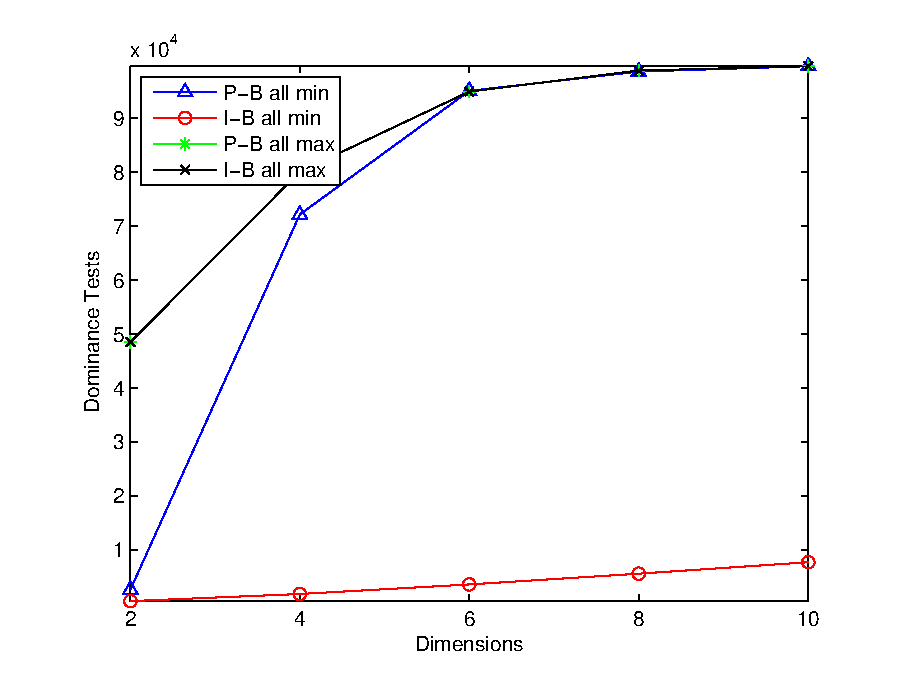
\includegraphics[width=1.6in]{Figures/exp/dt_dim_allmin_allmax.eps}
    %\end{minipage}
    }
  \subfigure[\small Mixed Data Types]{
    \label{fig:dt_dim_b}
    %\begin{minipage}[h!]{0.5\textwidth}
      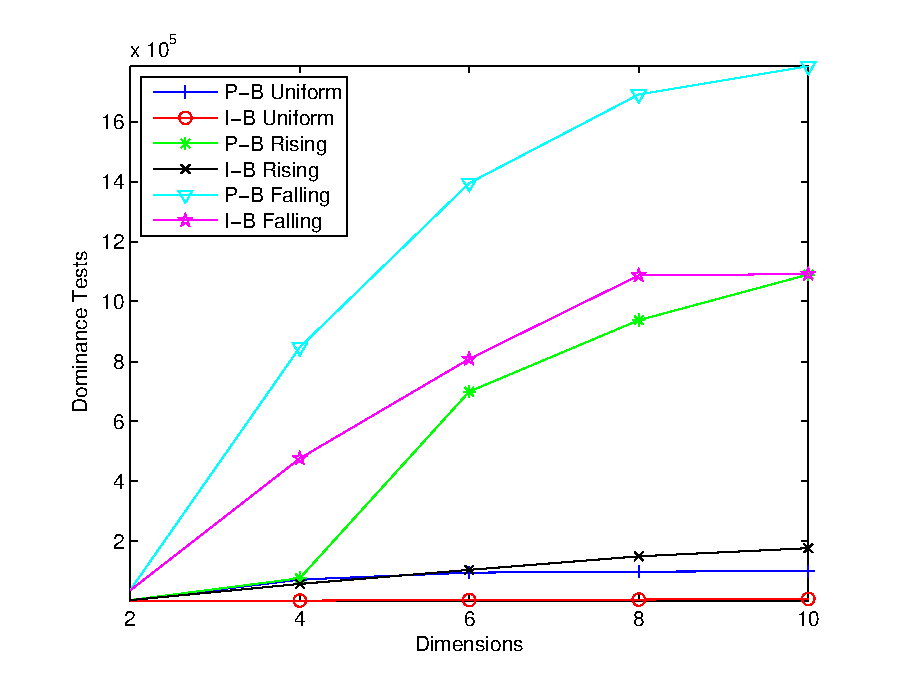
\includegraphics[width=1.6in]{Figures/exp/dt_dim_mixdata_rc10000.eps}
    %\end{minipage}
    }
  \caption{\small Dominance Tests vs. Dimensions. rc = 10000, b = 10}
  \label{fig:dt_dim}
\end{figure}


\subsection{Tuning Time}\label{sec:exp_tuning_time}

As discussed in section~\ref{sec:wireless_broadcast}, tuning time is total
amount of data the client has to download to fulfill a skyline query and
it is measured in bytes. The experiment simulates the server creating the
DFDI broadcast program. Tuning time is found by simulating a client evaluating
a skyline query from the beginning of the cycle.

Figure~\ref{fig:tt_rec} illustrates tuning time versus increasing record count
for all combinations of min and max attribute for 2-dimensional data. In
all cases, the Index-Based (I-P) pruning strategy performs several factors
better than Point-Based (P-B) pruning strategies.

Figure~\ref{fig:tt_dim} illustrates the simulation result for tuning time with
increasing data dimension. The experiments are run with record count (rc) of
10000, and branching factor (b) of index tree of 10.
Although the number of record stays the same, each additional dimension or
data attribute of the data-set adds space complexity to the data-set. With
increasing increasing dimensionality, the cycle length also increases, so
tuning time.

%%
% Tuning Time vs. Record Count
%%
\begin{figure}
  \centering
  \subfigure[\small (min, min) and (max, max)]{
    \label{fig:tt_rec_a}
    %\begin{minipage}[h!]{0.5\textwidth}
      \includegraphics[width=1.6in]{Figures/exp/tt_rc_minmin_maxmax.eps}
    %\end{minipage}
    }
  \subfigure[\small (min, max) and (max, min)]{
    \label{fig:tt_rec_b}
    %\begin{minipage}[h!]{0.5\textwidth}
      \includegraphics[width=1.6in]{Figures/exp/tt_rc_minmax_maxmin.eps}
    %\end{minipage}
    }
  \caption{\small Tuning Time vs. Record Count. d = 2, b = 10}
  \label{fig:tt_rec}
\end{figure}

%%
% Tuning Time vs. Dimension
%%
\begin{figure}
  \centering
  \subfigure[\small All Min and All Max]{
    \label{fig:tt_dim_a}
    %\begin{minipage}[h!]{0.5\textwidth}
      \includegraphics[width=1.6in]{Figures/exp/tt_dim_allmin_allmax_mod.eps}
    %\end{minipage}
    }
  \subfigure[\small Mixed Data Types]{
    \label{fig:tt_dim_b}
    %\begin{minipage}[h!]{0.5\textwidth}
      \includegraphics[width=1.6in]{Figures/exp/tt_dim_mixdata_rc10000.eps}
    %\end{minipage}
    }
  \caption{\small Tuning Time vs. Dimensionality. rc = 10000, b = 10}
  \label{fig:tt_dim}
\end{figure}

%%
% Index Percentage
%%
\begin{figure}
  \centering
  \subfigure[\small IP vs. Record Count]{
    \label{fig:ip_rc}
    %\begin{minipage}[h!]{0.5\textwidth}
      \includegraphics[width=1.6in]{Figures/exp/ip_rc.eps}
    %\end{minipage}
    }
  \subfigure[\small IP vs. Dimensionality]{
    \label{fig:ip_dim}
    %\begin{minipage}[h!]{0.5\textwidth}
      \includegraphics[width=1.6in]{Figures/exp/ip_dim.eps}
    %\end{minipage}
    }
  \caption{\small Index Percentage. b = 10}
  \label{fig:ip}
\end{figure}


\subsection{Index Percentage}

Index percentage measures the efficiency of the DFDI broadcast program
allocation technique under increasing record count and increasing data
dimension. Index percentage is defined in
section~\ref{sec:wireless_broadcast}.

Figure~\ref{fig:ip_rc} shows index percentage versus increasing record
count. For the DFDI, the simulation is run with replication level of 2,
which means the root and the first level below the root are replicated.
For the (1, m) index, m = 2, meaning the complete index is duplicated
2 times in the broadcast cycle.
The figure shows that the overhead of the index is high when the
number of record is low, but the overhead flattens as the number of
records grow. The one-time index is the baseline and as expected has
the lowest index percentage. Although DFDI replicated the index for
2 levels, its index percentage is only slightly (16\%) higher than
one-time index. This shows DFDI is efficient in terms of space
overhead. Whereas the (1, m) index has far worse overhead for only
2 duplications.

Figure~\ref{fig:ip_dim} shows index percentage over increasing data
dimension. The experiment is conducted with 10000 records and branching
factor of 10. As the data size grows with the number of dimensions, the
index is only slightly affected by the growth. The size of index grows
because of the index needs extra information to index the extra
dimensions, but the tree height is largely unaffected; thus gives the
falling of index percentage with growing dimension.

%Simulate 3 algorithms:
%\begin{enumerate}
%\item R-Tree one-time index \item R-Tree DFDI \item Grid R-Tree
%DFDI
%\end{enumerate}

%Measurements:
%\begin{enumerate}
%\item Index percentage (with variable branching factor) \item
%Tuning time (with variable branching factor) \item Dominance tests
%(with variable branching factor)
%\end{enumerate} 

\section{Related Work}\label{sec-related}

\subsection{Skyline Computation}

Techniques of computation of skyline records in traditional
database systems have been studied in \cite{skyline_operator},
\cite{shooting_stars}, and \cite{progressive_skyline}. The well
known algorithms are Nest-Loop, Block-Nested-Loop, and Divide and
Conquer. The Nest-Loop algorithm is an intuitive way to compute
skyline points in the way that every record is compared with every
other records in a table to determine if the record is dominated.
In Block-Nested-Loop, a record is only compared with other records
in the same block. The candidate skyline points in each block is
compare to obtain the final skyline points. In Divide and Conquer
(D\&C), the data set is recursively divided until there are only
two records. Skyline points are calculated for each segment
produced in the division phase. The division phase is followed by
a merge phase in which the skyline of all divisions are compare
and merge to obtain the final skyline set.

\cite{shooting_stars} introduces an online skyline computation
algorithm in which the skyline are computed progressively. The
first skyline is return almost immediately and more skyline points
are added to the result set.

Nearest Neighbor (NN) and Branch-and-Bound (BBS) skyline
algorithms are two of the best performing algorithms for
progressive skyline computation for traditional database systems
presented in \cite{progressive_skyline}. In NN skyline algorithm,
the records of the data set are presented geometrically in a
Euclidean space with the relevant attributes as the coordinate in
each dimension. In the example of hotel close to the ocean in
previously presented, a record would be placed on a plane with the
distance of the hotel to the ocean and its price as the two axis
that determine and the values in the two attributes as the
coordinates of the records on the Euclidean plane as in Figure
\ref{fig:skyline_nn}. The NN algorithm finds a nearest neighbor
from the axes and that is the first skyline point. Then the
algorithm marks the region that is dominated by the first skyline
point so that anything in that region will not be searched. The
search results in two more search regions and the search continues
until no more records are left.

\begin{figure}[h]
\begin{center}
\includegraphics[width=2in]{Figures/skyline_nn.eps}
\caption{\small NN d and its pruning region.
\label{fig:skyline_nn}}
\end{center}
\end{figure}

BBS is an algorithm that surpass the computation efficiency of the
NN algorithm. BBS utilizes the best first search technique to
traverse the index tree to prune the branches unnecessary
branches. Unfortunately, both NN and BBS can not be easily adopted
to the broadcast environment due to the linear nature of broadcast
program. Both NN and BBS requires backtracking of the index tree
to find the best path to prune, which is impermissible in
broadcast environment or require waiting for the next broadcast
cycle, which incurs long waiting time. The solutions presented in
this paper will use the pruning regions strategy used in NN. Our
algorithms systematically builds pruning regions, as presented in
NN algorithm, as the client receives and discovers more data from
the broadcast channel.


\subsection{Wireless Broadcast Index}\label{sec:wireless_bcast_index}
Many excellent studies have been done on improving efficiency of
wireless broadcast system using indexing techniques. This section
considers several popular index allocation techniques and
discusses benefits and drawbacks.

The intuitive technique of no index and one-time index at
beginning of a broadcast cycle has been considered in
\cite{data_on_air}. With no index, the length of a cycle is
minimized, but the tuning time is the entire cycle since the
program is not self-descriptive. With one-time index, the clients
are able to filter unwanted data and reduce tuning time, but if a
client misses the one-time index, then it will have to wait until
the next cycle even if there is useful data in current cycle.

$(1, m)$ indexing, proposed by Imielinski, et al. in
\cite{data_on_air}, is a mitigation to the problem of one-time
index by replicating the entire index every $1/m$ length of the
broadcast cycle. The benefit of this index technique is when a
client misses an index segment, it can wait for the next index in
the same cycle \cite{DBLP:journals/tmc/KuZW08}. The drawback of
this technique is the space consumption of replicating the full
index several times in the cycle.

Distributed index was also proposed in \cite{data_on_air}. This
index also replicate the index in the broadcast cycle, but only a
part of the index is replicated. Advantages of this method are (1)
index can be obtained throughout cycle, (2) reduced bandwidth
consumption comparing with $(1, m)$, and (3) not limited to
particular index structure.

%\cite{data_on_air} by Imielinski, et al. is an
%early and influential work of data
%indexing for broadcast on air. The paper defined two
%characteristics of wireless broadcast, \em{tuning time} and \em{access latency}. Tuning time
%defines how long the client has to actively listen on the channel to get all the desired data.
%Access latency define the time when the client issues the query to the time all the desired
%data is received. Tuning time is proportional to power usage of mobile clients. The goal is to
%reduce both tuning time and access latency.

%In addition, the paper also proposed a few air index techniques to reduce client tuning time.
%The first index proposed is $(1, m)$ index, in which the full index is repeated every $1/m$ of
%the entire broadcast cycle. The index is repeat so that clients that tune into the channel in
%the middle of the broadcast does not have to wait until the next cycle to get the index and
%process request. The second index proposed is the distributed index, in which only a part of
%the index is repeated. Distributed index reduces the overhead of embedding index and improves
%access latency.

Data filtering based on data signature was proposed in
\cite{signature_and_caching}. During data retrieval, the signature
of desire data is compared with the signature of a data segment
prepared by the broadcast server. If the signatures match, then
data is downloaded, else ignored.

Distributed index for spatial data in error-prone air broadcast
was introduced in \cite{dsi}. Instead of replication, his paper
proposes a distributed index in the broadcast cycle with no
duplicate of index. The paper index broadcast spatial data using
Hilbert values. Each data record contains an index table that
contains the data segments that will be pushed onto the channel in
the near future. A drawback of this approach is the lose of
spatial precision due to the use of space filling curve as index.


%\section{System Model}

%In our theoretical model, the system consists of the broadcast server and multiple clients. As
%discussed in section 2.1, the server periodically broadcast data in a specific channel. Any client
%that is interested in any of the data serviced by the server tunes into the channel to get the
%desire data. The server contains a set of records as illustrated in Figure 4.

%In this model, we assume a pure broadcast model in which all data are transmitted through downlink
%bandwidth and that there is not uplink bandwidth. Clients must tune into the channel as long as it
%takes to obtain all desire data. Apparently, in order to support efficient query, the server must
%provide data index so that the client can tune in only when the relevant data is to be broadcasted
%In addition, this model contains only one transmission channel. Index must be transmitted on the
%same channel as the data.


\section{Conclusion}\label{sec-conc}
In this paper, we presented a broadcast data stream allocation technique
(DFDI) that utilize the R-Tree and performs a depth-first traversal of the
index to create a distributed index. The goal of DFDI are to facilitate
query processing from broadcast data, to reduce index overhead (IP) and,
to improve the initial index prob. DFDI is able to achieve all these with
reasonable efficiency. DFDI is a flexible R-Tree based index and
well-supports skyline queries as well as other data query types. The allocation
distributes $b^h$ number of index segments among the broadcast program to
reduce initial index at the same time keeps the index overhead low. The simulation
results for index percentage show DFDI performs very well with 2 levels of
replication and follow the efficiency of one-time index with only $16\%$
increase in index overhead.

The simulation result show that the approach also performs well with data
of higher dimensions. The index overhead decreases as the number of records
remain constant and the number of data dimension increase. This is due to
the growth of dimensionality does not make the index tree grow "taller" and
does not incur the cost of new nodes when the index grows. The height of
an index tree does increase as the number of records increase, but as seen
in Figure~\ref{fig:ip_rc}, the growth of the index is not as fast as the
growth of the amount of data; therefore, the index overhead decreases as
records increase.

In addition, we introduced point-based and index-based pruning skyline
algorithms. The experiments shows both algorithms are capable of evaluate
skyline queries of combined $min$ and $max$ attributes with reasonable
tuning time and dominance tests. The index-based skyline had
always performed better than the point-based skyline, in some cases several
factors. The performance of the algorithms is also affected by the data
arrangement and R-Tree implementation. From our simulation, we find that
R-Tree that index records with lower attributes first, performs better for
$min$ skyline queries, and vice versa.

\section*{Acknowledgements}
\input{ack}

%\small {\section*{Acknowledgments}


\bibliographystyle{abbrv}
\bibliography{bibliography}

\end{document}
